
\section{Page-aware template scoring}
\label{sec:gwes}

In the global page-aware context, template evaluation shifts from isolated single-article selection to assessing candidate template assignments across all articles assigned to a unified page canvas $\page$. This requirement stems from the fact that professional newspaper layouts exhibit tacit structural and visual dependencies, where selecting a template $\templatesel{i}$ for a given article $\articleobj{i}$ inherently depends upon, and influences, the spatial arrangement, aspect ratio, and editorial hierarchy of neighboring articles on the same page canvas.

Evaluating template suitability at the page level requires simultaneously addressing two complementary factors: modeling the internal topological structure of individual templates and capturing the contextual interdependencies among the set of articles $\articleset = \{\articleobj{1}, \articleobj{2}, \dots, \articleobj{n}\}$ co-existing on the page. Standard flat metadata metrics and independent ranking mechanisms are insufficient for this task because they evaluate candidate templates in isolation, failing to capture how spatial configurations interact across adjacent layout blocks to form a cohesive visual spread.

%%%%%% From here keep it
Rather than relying on rigid, handcrafted heuristic rules that fail to capture the nuances of human design, this challenge is addressed by developing a neural evaluation metric that scores the quality of assigned templates $\templatesel{i}$ for each article $\articleobj{i}$ in the page $\page$, considering also their placement in the canvas. This module dynamically scores the contextual harmony between an article's content and its spatial configuration within a newspaper layout, combining a dynamic sequence-level Transformer encoder with a precalculated topological template similarity matrix (using $\gmn{\cdot}{\cdot}$) into a single neural method coined \NeuralMethod\ (\neuralmethod).



\subsection{Problem formulation}
\label{sec:gwes-problem-formulation}

When an article is instead evaluated as part of a page canvas $\page$ shared with other articles $\articleset = \{\articleobj{1}, \dots, \articleobj{n}\}$, editorial harmony between neighboring templates is the goal. 

Formally, the input to this setting is a page canvas $\page$ populated by the article set $\articleset$, each article $\articleobj{i}$ already carrying a candidate template assignment $\templatesel{i}$; this setting is therefore formalized as scoring, rather than retrieving, the compatibility of this joint assignment, conditioned on each article's neighbors on the page. 

Given this formalism, the desired output is a compatibility matrix $\mathbf{P} \in [0,1]^{\numarticles \times \catalogsize}$, where each entry expresses the contextual suitability of assigning a given catalog template to a given article, conditioned on the rest of the page. These per-article scores are later combined with the template similarity matrix $\gmnMatrix$ (\secref{sec:gwes-gmn-mapping}) into a single scalar \neuralmethod\ score for the whole layout $\solution$.

\subsection{Proposed approach}

\neuralmethod\ addresses this problem by combining a Transformer-based encoder, which scores contextual editorial suitability, with the topology-aware similarity metric $\gmn{\cdot}{\cdot}$, which corrects that score for long-tail bias.

\subsubsection{Transformer-based Editorial Intent Module}
\label{sec:transformer_module}

The primary role of the Transformer-based encoder is to operate as a contextual network that scores the appropriateness of each template $\templatesel{i}$ given the specific metadata of each article $\articleobj{i}$ in the set of placed articles $\articleset$ (of size $\numarticles$) and their placement on the page canvas $\page$. Unlike static classification networks, this encoder evaluates the entire page context simultaneously, capturing how the spatial configuration of one article influences the editorial validity of its neighbors.

\paragraph{Input Tensor}

To feed the joint article-template assignment $(\page, \articleset)$ into the Transformer encoder, the article set $\articleset$ (together with each article's currently assigned template $\templatesel{i}$) is reformatted into a single input tensor, aggregating three distinct feature streams per article:
\begin{enumerate}
    \item \textbf{Input Metadata ($\mathbf{m}_i$):} The intrinsic structural features of article $\articleobj{i} \in \articleset$ exactly as defined in Chapter~\ref{chapter:definitions}. This vector encapsulates four concrete numerical features extracted from the input instance: the body text character count, the total number of allocated images, and binary flags indicating the presence of an article title and subtitle, respectively.
    
    \item \textbf{Spatial Coordinates ($\mathbf{c}_i$):} The absolute geometric coordinates of each article $\articleobj{i} \in \articleset$, relative to the page dimensions (\Wpage\ and \Hpage). This vector captures the physical bounding box properties of $\articleobj{i}$, specifically its top-left grid coordinates $(x_i, y_i)$, width $\Wtemp{\templatesel{i}}$, and height $\Htemp{\templatesel{i}}$.
    
    \item \textbf{Template Zoning ($\zoning{i}$):} A flattened structural vector aggregating the internal geometric coordinates of all constituent blocks within template $\templatesel{i}$. For each zoning block $\zblock{i}{k} \in \zoning{i}$, a 5-dimensional feature tuple is appended to the vector, corresponding to a numerical identifier of the semantic feature class $\blockfeat{\zblock{i}{k}}$ (as formalized in Chapter~\ref{chapter:definitions}), followed by its relative bounding box properties $(x, y, w, h)$ normalized by the template dimensions $\Wtemp{\templatesel{i}}$ and $\Htemp{\templatesel{i}}$. This representation captures the layout topology of the template.


\end{enumerate}


For each individual article $\articleobj{i}$, the feature streams are concatenated into a unified vector $\mathbf{x}_i \in \mathbb{R}^{109}$, where the template zoning window is zero-padded up to its maximum  capacity. To evaluate the entire layout as a cohesive unit, the vectors of all $\numarticles$ active articles are sorted from top-to-bottom and left-to-right based on their top-left coordinates, and stacked into a sequence tensor. To accommodate variations in article counts across layouts, these sequences are uniformly padded, while a boolean mask isolates the active articles to evaluate the global page context simultaneously.

\paragraph{Transformer Encoder Model}

The sequence of article vectors $\mathbf{x}_i \in \mathbb{R}^{109}$ representing the layout are subsequently and simultaneously fed into the network. First, a dense linear projection layer maps the 109-dimensional feature space into a 128-dimensional latent embedding space:

\begin{equation}
\mathbf{h}_i^{(0)} = \text{GELU}(\mathbf{W}_p \mathbf{x}_i + \mathbf{b}_p)
\end{equation}
where $\mathbf{W}_p \in \mathbb{R}^{128 \times 109}$ and $\mathbf{b}_p \in \mathbb{R}^{128}$ denote the projection weights and biases, and a Gaussian Error Linear Unit (GELU) activation function introduces non-linear activation thresholds to capture complex editorial compliance patterns. 


To capture the structural hierarchy and sequential sorting order of articles on the page, a learnable positional embedding is additively combined with the projected representations based on each article's sequence index.

This sequence of tokens is subsequently passed to a Transformer encoder~\cite{attention} stack comprised of 4 layers and 8 parallel self-attention heads, with a 512-dimensional feed-forward network. A standard padding mask is applied to restrict the multi-head self-attention mechanism exclusively to the active articles in $\solution$.

Finally, the output of the encoder stack passes through a linear classification softmax layer to generate a probability matrix of dimensions $\numarticles \times \catalogsize$. Each entry in this matrix defines the contextual suitability, expressed as a probability $p\in[0,1]$ of a specific template for a given article in the page layout. 

\subsubsection{tGMN inclusion for template similarity}
\label{sec:gwes-gmn-mapping}

While the Transformer encoder models the dynamic suitability of template assignments based on historical contexts, it is inherently susceptible to long-tail bias, leading to the frequent under-scoring of valid templates simply because they are under-represented in the historical training dataset. This will cause that even if the Transformer achieves high predictive accuracy, its raw probability distributions might be highly concentrated, creating a rigid search space that can cause evolutionary operators to stall. 

To mitigate this, \neuralmethod\ incorporates a precalculated pairwise similarity matrix $\gmnMatrix = [s_{ij}] \in \mathbb{R}^{\catalogsize \times \catalogsize}$ derived from $\gmn{\cdot}{\cdot}$ and $\gmnNetwork$~\cite{patil_layoutgmn_2021, li-gmn-2019}.

However, and because the raw score $\gmn{\cdot}{\cdot}$ is unbounded ($\gmn{\templateobj{i}}{\templateobj{j}} \in (0, \infty], \forall i,j$), these values are mapped into a normalized affinity range $[0,1]$ using a Gaussian kernel transformation:
\begin{equation}
s_{ij} = \exp\left( -\frac{\gmn{\templateobj{i}}{\templateobj{j}}^2}{2(\sigmagmn)^2} \right)
\end{equation}
where $\sigmagmn$ represents a scaling parameter set according to the dataset characteristics to control the smoothness of the topological mapping. This transformation yields the final similarity matrix $\gmnMatrix$, with a bounded similarity score $s_{ij} \in [0, 1]$ between any pair of templates.

\subsubsection{\NeuralMethod (\neuralmethod)}

Finally, to obtain the \neuralmethod, the probabilities from the Transformer and the topological affinities from $\gmnMatrix$ must be algebraically combined. 

Let $\mathbf{P} \in [0,1]^{\numarticles \times \catalogsize}$ be the probability matrix output by the Transformer encoder, where $p_{i,k}$ represents the contextual suitability of assigning template $k$ to article $\articleobj{i}$. Concurrently, let $\templatesel{i} \in \{1, \dots, \catalogsize\}$ denote the  template assignment for said article. The localized compatibility score $\alpha_i$ for article $\articleobj{i}$ is formalized as the dot product between the article's probability distribution and the topological similarity profile of the selected template:
\begin{equation}
\alpha_i = \sum_{k=1}^{\catalogsize} p_{i,k} s_{\templatesel{i}, k}
\end{equation}
where $s_{\templatesel{i}, k}$ is the similarity between the selected template $\templatesel{i}$ and any catalog template $k$, retrieved directly from $\gmnMatrix$. 

This formulation mathematically expresses the probability ``smoothing'' mechanism: if an algorithm or a designer selects a rare template $\templatesel{i}$ that suffers from long-tail bias in the Transformer (yielding a low $p_{i,\templatesel{i}}$), $\alpha_i$ will remain high as long as $\templatesel{i}$ shares a high topological similarity with other frequent templates that received robust probabilities. Finally, to align this metric with a minimization paradigm (necessary for the following chapters), the page-level \NeuralMethod\ (\neuralmethod) score for a layout $\solution$ is aggregated as an editorial mismatch penalty:
\begin{equation}
\neuralmethod(\solution) = \sum_{i=1}^{\numarticles} (1 - \alpha_i)
\end{equation}

\subsection{Experimental evaluation}
\label{sec:gwes-evaluation}

In this section the predictive capabilities and structural behavior of the components underlying the \neuralmethod\ metric are verified. 

\subsubsection{Implementation and Hardware Details}
\label{sec:gwes-implementation}

All deep learning pipelines are powered by the \textit{PyTorch}~\cite{pytorch} ecosystem. This neural framework encompasses the dynamic sequence-level Transformer encoder responsible for predicting historical editorial intent, alongside the implementation of the Layout Graph Matching Network (GMN) utilized to calculate the pre-computed topological affinity matrix~$\gmnMatrix$.

The  training phase for the Transformer Encoder was conducted on a dedicated high-performance GPU computing cluster node, powered by an Intel Xeon Silver 4110 processor, 96~GB of system RAM, and an NVIDIA Tesla T4 GPU with 15~GB of dedicated video memory (VRAM).

\subsubsection{Page Layout and Template Catalog Dataset}

To evaluate the architectural robustness and industrial applicability of the proposed framework, empirical validations were conducted using the available \laprovence archive (\secref{sec:laprovence}). The historical page dataset  provides the required historical context to train the Transformer Encoder module of \neuralmethod. Concurrently, the static template catalog~$\templatecatalog$ serves as the underlying structural dataset utilized to compute the $\gmnMatrix$ matrix.

\paragraph{Historical Layout Dataset}

The historical layout dataset contains a total of $6,007$ production pages extracted from the publisher's workflows. To establish a high-fidelity benchmark, a data-cleaning pipeline was deployed to isolate incomplete or deformed layout files, resulting in $4,449$ fully usable, non-corrupted pages. 

Each layout instance in this clean repository is represented as a detailed XML file encapsulating three data streams:
\begin{itemize}
    \item The global physical dimensions of the page canvas~$\page$, specifying total nominal boundaries ($\Wpage, \Hpage$) and margins ($\mtop, \mbottom, \mleft, \mright$).
    \item The exact top-left coordinate placements ($\xcoord{i}, \ycoord{i}$), dimensions for each individual article~$\articleobj{i}$ relative to the page origin, and the assigned template $\templatesel{i}$.
    \item A structural copy of the internal zoning topology~$\zoning{\templatesel{i}}$, outlining the relative bounding shapes and semantic feature classes of the inner blocks belonging to the chosen template~$\templatesel{i}$.
\end{itemize}

The final dataset consider instances containing a variable count of between $1$ and $11$ distinct news articles arranged simultaneously within a single page canvas.


\paragraph{Template Catalog}

The structural template catalog $\templatecatalog$ is composed by  $\catalogsize = 345$ designs from \laprovence archive. Each blueprint specifies all elements described in Chapter~\ref{chapter:definitions} for a given template: dimensions ($W_j, H_j$), internal zoning $\zoning{j}$ and text capacity mapping $\capacity{j}$. 


\subsubsection{$\gmnMatrix$ calculation}

The structural similarity matrix $\gmnMatrix$ is computed utilizing the template catalog $\templatecatalog$ from \laprovence, but using an instance of $\gmnNetwork$ pre-trained on the analogous, structurally equivalent publishing corpus of \publihebdos, detailed in \secref{section:trs-eval}. 

This calculation outputs a matrix with dimensions $\gmnMatrix = [s_{ij}] \in \mathbb{R}^{345 \times 345}$. Consequently, the training validation and convergence analyses presented in the following sections focus exclusively on the Transformer Encoder architecture. $\gmnMatrix$\  assumes a prominent role  within the evaluation of the unified \neuralmethod\ metric.


\subsubsection{Transformer Encoder Training Hyperparameters}
\label{subsec:hyperparameter_calibration_transformer}

The operational parameters governing the neural training of the Transformer Encoder in \neuralmethod\  were set through extensive empirical pilot studies over the specified dataset. 

The finalized parameters are structured in Table~\ref{tab:algorithmic_parameters_transformer}.

\begin{table}[htbp]
\centering

\begin{tabularx}{\textwidth}{@{}l l X l@{}}
\toprule
Category & Symbol & Parameter Description & Value \\
\midrule
\multirow{7}{*}{\makecell[l]{Transformer \\ Encoder Training}}
           & --- & Neural optimizer architecture & AdamW \\
           & --- & Train/Val/Test split & $80\%/15\%/5\%$ \\
           & --- & Base learning rate & $10^{-4}$ \\
           & --- & Weight decay & $10^{-2}$ \\
           & --- & Batch size & 128 \\
           & --- & Total deep learning training epochs & 3000 \\
           & --- & Early stopping epoch threshold & 40 \\
\bottomrule
\end{tabularx}

\caption{Algorithmic and structural hyperparameters for the Transformer Encoder training.}
\label{tab:algorithmic_parameters_transformer}
\end{table}

\subsubsection{Dataset Split}
The filtered repository of $4,449$ usable pages was passed through a multi-label denoising and stratification pipeline. A global frequency census was executed across all pages to track template occurrences. To ensure that the subsequent split remains mathematically viable for stratified multi-label partitioning, a minimum threshold of three global samples per template class was enforced, guaranteeing adequate representation across the training, validation, and testing folds. Consequently, $67$ pages (representing $1.51\%$ of the corpus) containing orphan or ultra-rare template configurations were removed. 

The remaining $4,382$ production pages were partitioned using an iterative multi-label stratification algorithm with the split ratio indicated in Table~\ref{tab:algorithmic_parameters}. 

\subsubsection{Training Convergence}

The model was trained using cross-entropy loss over a maximum of $3,000$ epochs with an early stopping threshold of $40$ epochs. 

\begin{figure}[htbp]
\centering
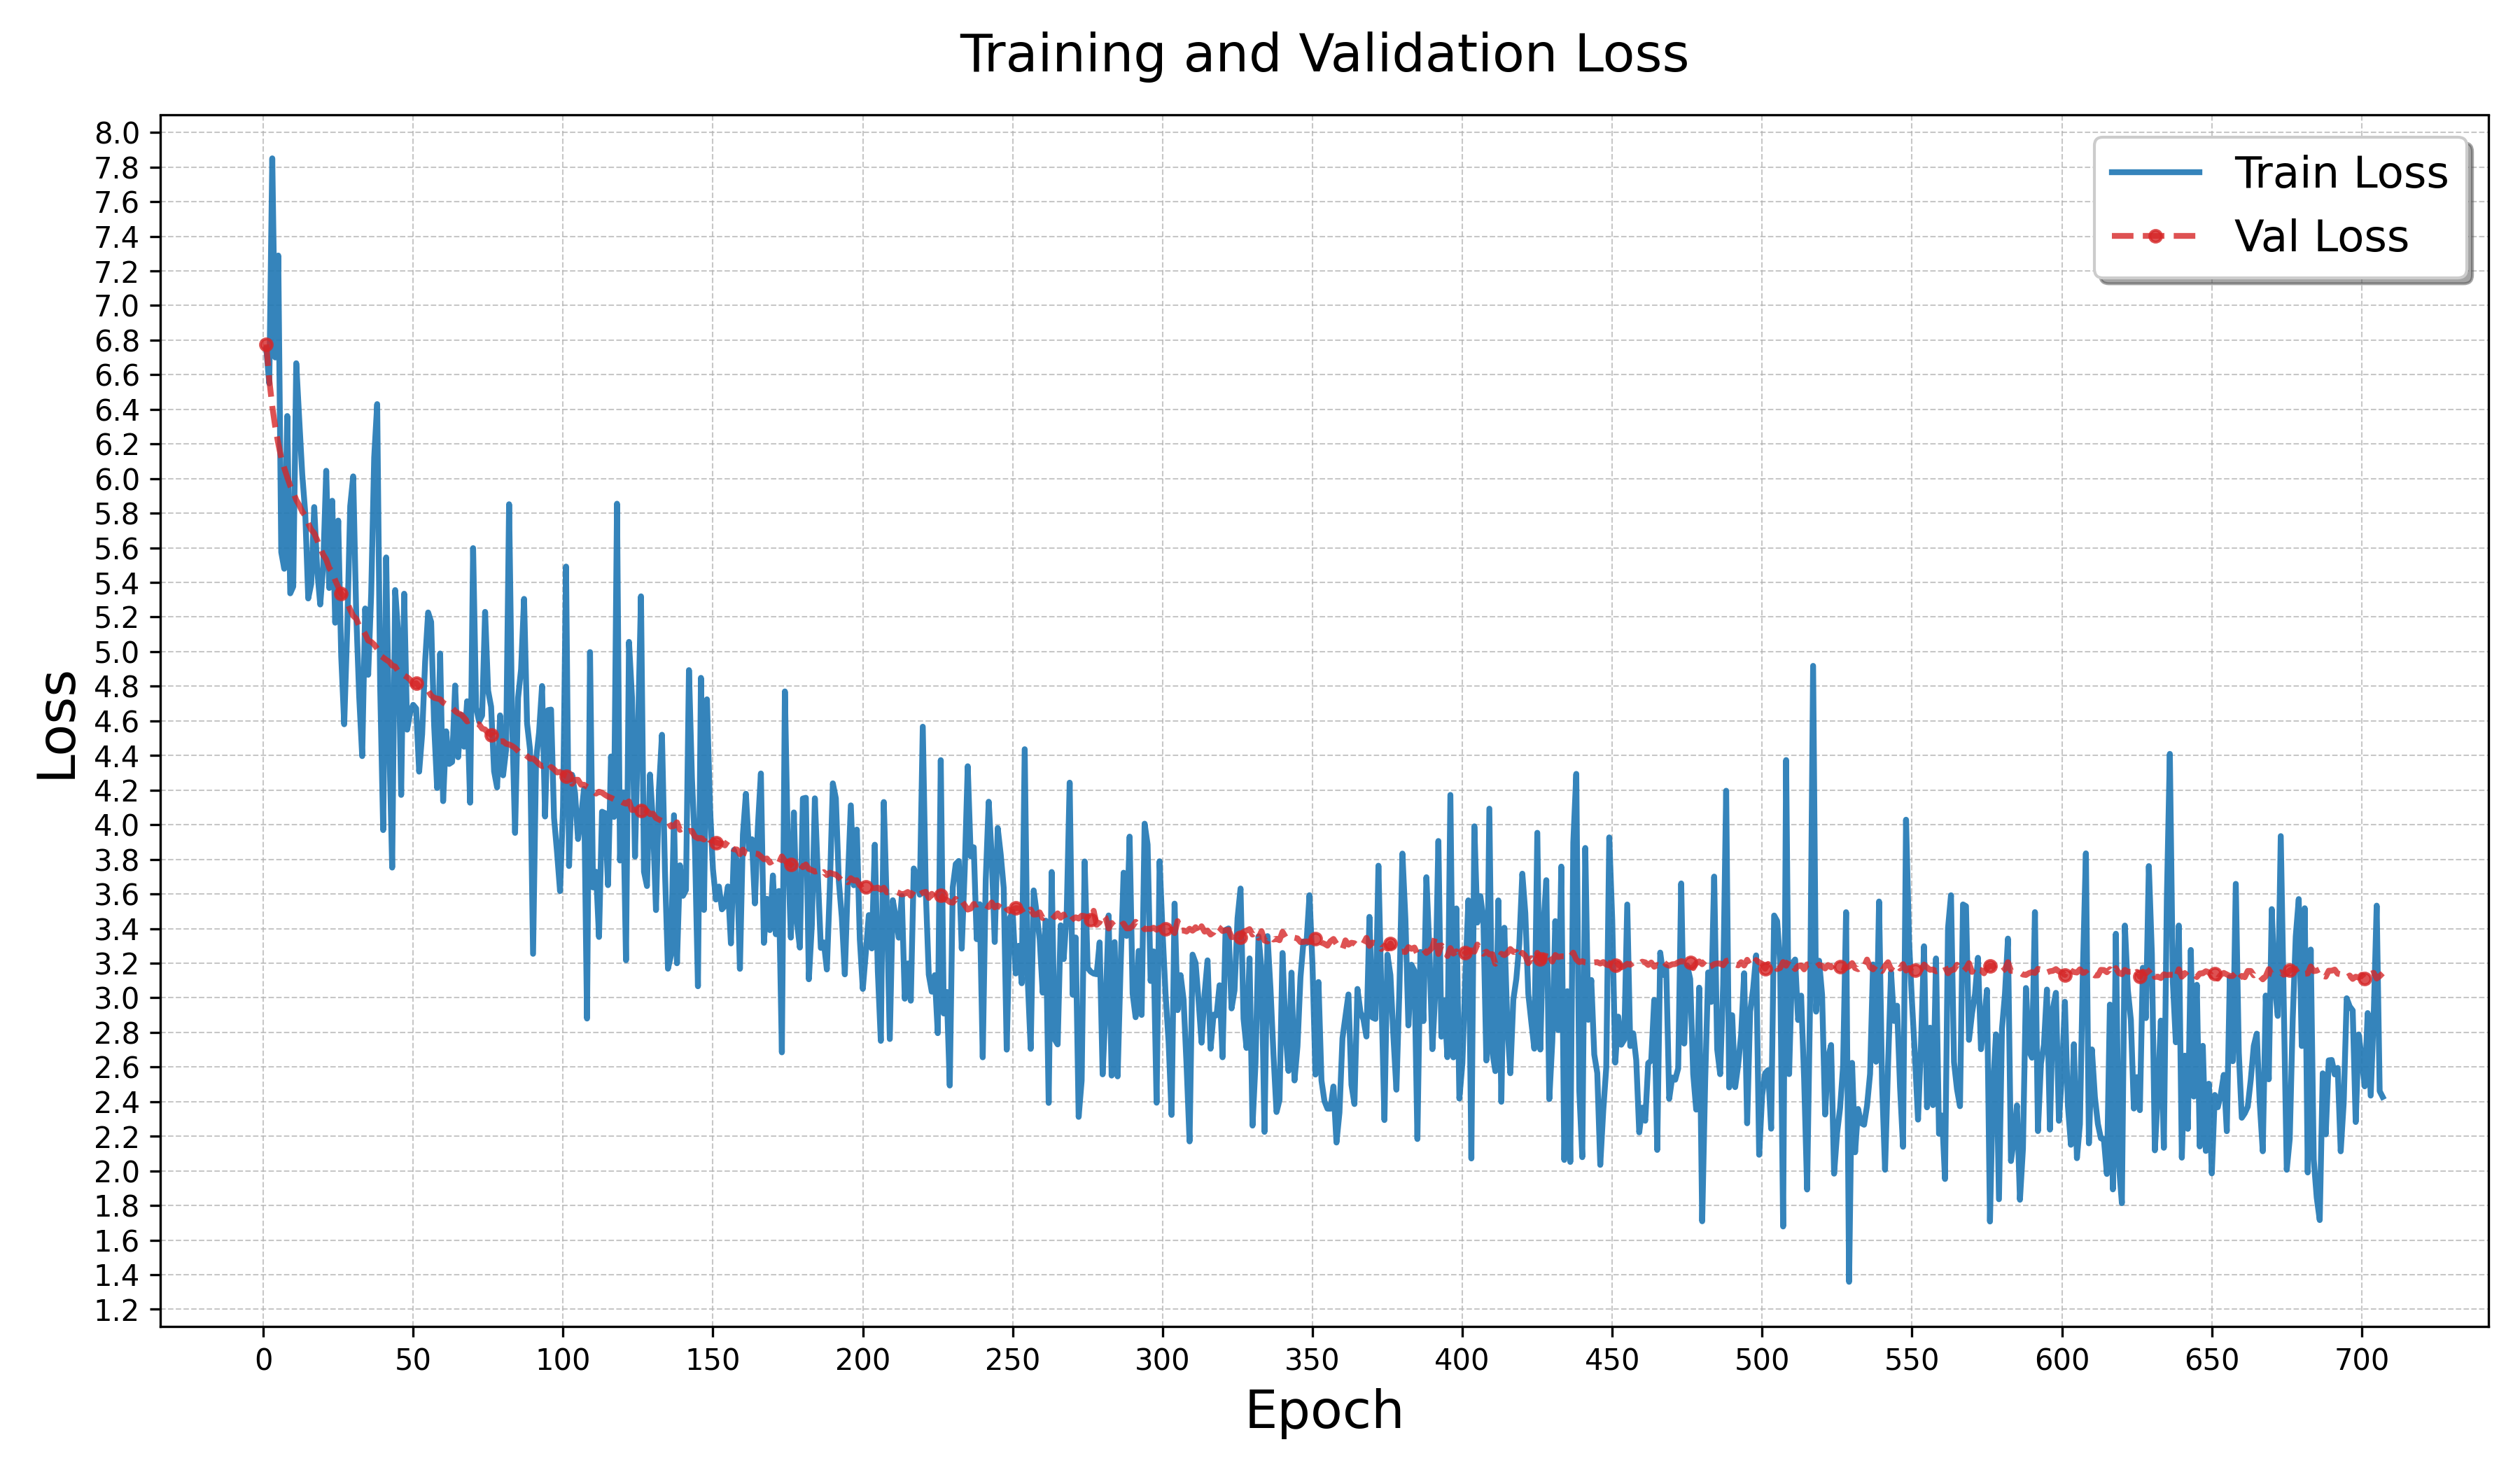
\includegraphics[width=\widthForOneImage]{img/loss_curve.png}
\caption{Training and validation loss curves across optimization epochs.}
\label{fig:loss-curves}
\end{figure}

As illustrated in \figref{fig:loss-curves}, the  oscillations observed in the training loss curve are driven by the intentional feature-dropout protocol applied to the spatial coordinates and zoning matrices during the forward training pass, which introduces controlled batch-level variance. Conversely, during the validation phase, this is not the case and the curve is exceptionally smooth. 

The stabilization of the validation loss at approximately $3.1$ reflects the intrinsic ambiguity of selecting a single exact template from a domain of $\catalogsize = 345$ choices, where multiple configurations can be equally appropriate for the same content. Because cross-entropy heavily penalizes this, the validation loss serves primarily as an internal training convergence guide. Consequently, the true evaluation of the network's performance shifts to the Top-$K$ accuracy rates over the test set and subsequent ablations.


\subsubsection{Predictive Top-K Performance and Feature Ablation}

The dataset split process yielded a definitive test set consisting of $232$ high-fidelity production pages encompassing $587$ individual news articles.

To evaluate both the predictive accuracy and the relative impact of each data stream within the input features, the Top-$K$ accuracy metrics were validated over this independent test set across two operational ablation scenarios: 
\begin{enumerate}
    \item \textit{Metadata Only}: Masking out all absolute coordinates and template zoning details (indices 4--109 reset to $-1.0$) to evaluate predictions based purely on content requirements. This configuration is used when no layout information is available.
    \item \textit{Full Context}: Utilizing the complete information stream, combining raw article metadata, physical coordinates, and internal template zoning topologies.
\end{enumerate}

In all scenarios, a prediction is certified as correct if the target template chosen by the original human designer matches one of the top $K$ highest-probability outputs generated by the softmax distribution. The comparative quantitative results are summarized in Table~\ref{tab:topk_ablation_accuracy}.


\begin{table}[htbp]
    \centering
    \begin{tabularx}{\widthForParametersTable}{Xccc}
    \hline
    \textbf{Available Context} & \textbf{Top-1 Accuracy} & \textbf{Top-3 Accuracy} & \textbf{Top-5 Accuracy} \\ \hline
    Metadata Only & 16.70\% & 35.60\% & 49.23\% \\
    Full Context & 82.62\% & 95.06\% & 97.61\% \\ \hline
    \end{tabularx}
    \caption{Multi-scenario Top-$K$ predictive accuracy and feature ablation rates over the independent test set ($232$ pages, $587$ articles).}
    \label{tab:topk_ablation_accuracy}
\end{table}


The comparative rates in Table~\ref{tab:topk_ablation_accuracy} validate the core assumptions of the hybrid architecture. While the metadata-only scenario exhibits a low Top-1 accuracy of 16.70\% due to the extreme structural ambiguity of predicting a layout without spatial boundaries, its Top-5 accuracy of 49.23\% confirms that the network successfully narrows down the massive search space of 345 designs into a highly relevant subset, providing a good bias for the initialization and mutation operators. Conversely, when the complete physical and zoning context is available, the model achieves an outstanding accuracy, proving that the relational self-attention mechanism successfully captures the latent rules of template assignment.


\subsubsection{$\gmnMatrix$ impact in \neuralmethod}

Although the standalone Transformer Encoder achieves high predictive accuracy, its raw probability distributions are often highly concentrated. To evaluate how the algebraic integration of the LayoutGMN affinity matrix~$\gmnMatrix$ relaxes this constraint boundary without destroying human design alignment, an exhaustive analysis was executed over the test set. 

This validation measures the smoothing effect of the unified \neuralmethod\ metric by capturing flexibility gains across the dataset. For absolute mathematical rigor, because the raw matrix multiplication $\gmnMatrix \cdot \mathbf{V}_{T}^{(i)}$ yields non-normalized structural affinity values, the score vectors were temporarily normalized for the statistical computation to ensure an equivalent probability density domain. This calibration is strictly analytical and restricted to the calculation of these metrics, allowing a fair baseline comparison. The quantitative results of this analysis are summarized in Table~\ref{tab:gmn_impact}.

\begin{table}[htbp]
\centering
\begin{tabularx}{\widthForParametersTable}{Xcc}
\hline
\textbf{} & \textbf{Transformer Only} & \textbf{GWES Resonance}  \\ \hline
Avg. Viable Options ($\text{Prob.} > 5\%$) & 1.89 & 3.23  \\
Max Confidence Peak ($\|\cdot\|_\infty$) & 0.62 & 0.18  \\ \hline
\end{tabularx}
\caption{Quantitative search space relaxation and normalized topological smoothing metrics on the test set ($232$ pages, $587$ articles).}

\label{tab:gmn_impact}
\end{table}

The metrics detailed in Table~\ref{tab:gmn_impact} confirm that the topological convolution step expands the average pool of viable layout alternatives from $1.89$ to $3.23$ options per article, yielding a stable 1.7$\times$ gain in search space flexibility. This phenomenon represents a controlled probability diffusion mechanism, where mass is transferred from isolated predictions toward geometric neighbors. Crucially, this diffusion actively counteracts predictor rigidity, achieving a $71.14\%$ reduction in the distribution's maximum confidence peak (with the mean infinity norm dropping from $0.62$ down to $0.18$). While this smooth distribution naturally lowers the absolute dominance of the top-1 template due to mass sharing among interchangeable designs (while maintaining top-1 rank dominance in general), it successfully transforms a highly polarized search space into a cooperative landscape suitable for optimization tasks.

\begin{figure}[htbp]
\centering
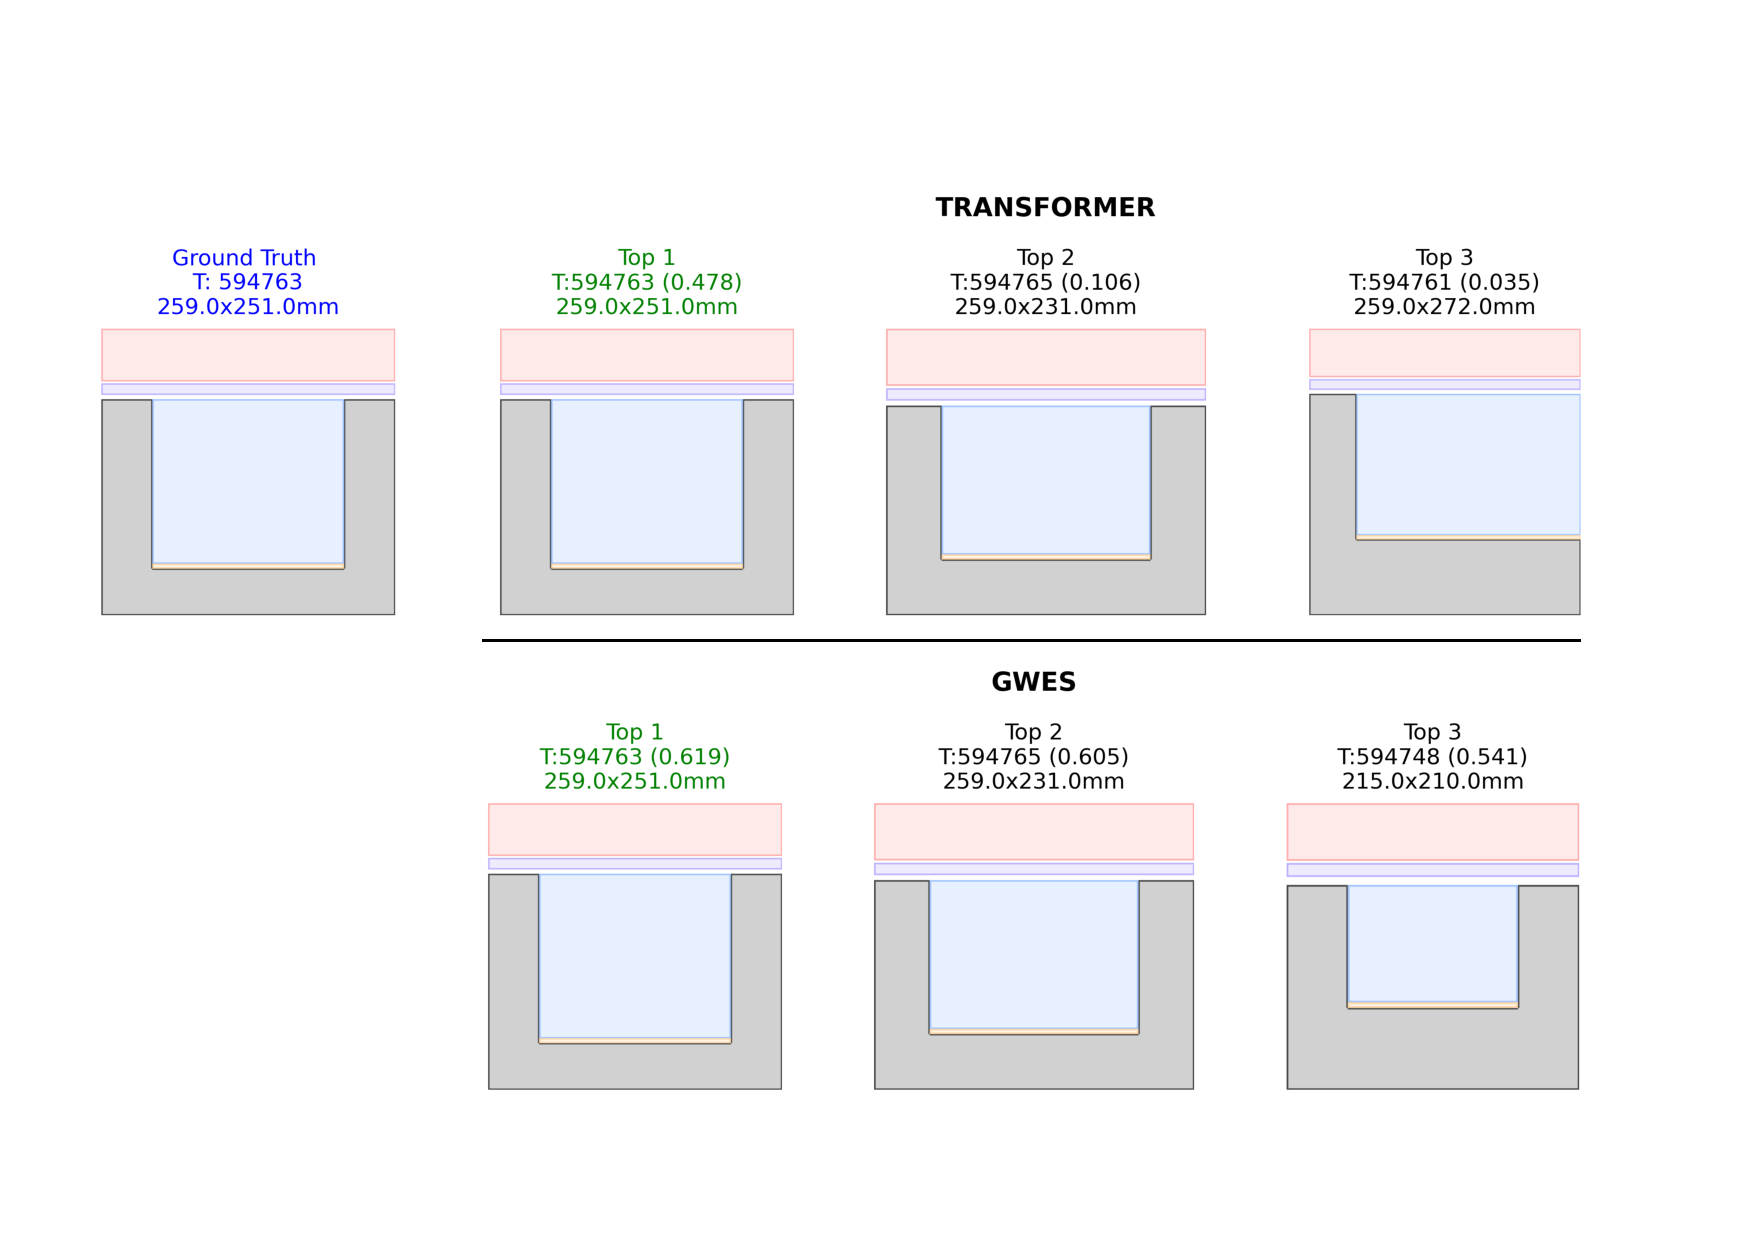
\includegraphics[width=\widthForOneImage]{img/gwes_vs_transformer_ex2.pdf}
\caption{Qualitative behavior of $\gmnMatrix$ smoothing of the Transformer Encoder, for a ground truth target (in blue). Green labels denote the target template. While the raw Transformer pipeline (top row) operates over a formal probability distribution summing to unity, the integrated \neuralmethod\ framework (bottom row) maps raw, non-normalized structural affinity scores derived from the matrix multiplication with $\gmnMatrix$. }
\label{fig:gwes-vs-transformer}
\end{figure}


This behavioral characteristic is qualitatively illustrated in \figref{fig:gwes-vs-transformer}. As shown in this representative example, the human-selected target template (\texttt{T:594763}) is successfully identified as the top rank by both paradigms. However, the standalone Transformer exhibits a rigid, steep probability drop-off immediately after its first choice, collapsing from $0.478$ down to $0.106$ and $0.035$ for the subsequent positions. This polarization penalizes structurally similar alternatives, severely limiting the exploration capacity of the evolutionary engine if the top candidate encounters conflicts.


Conversely, the unified \neuralmethod\ metric leverages the graph-matching prior to build a cooperative, high-utility plateau. To reflect the true operational reality of the evolutionary process, the values displayed for \neuralmethod\ in \figref{fig:gwes-vs-transformer} correspond to the raw, non-normalized affinity scores rather than formal probabilities. Under this framework, \neuralmethod\ actively expands the search space by shifting values; the target template achieves a dominant affinity score of $0.619$, while its direct visual twin (\texttt{T:594765}) is elevated to an equivalent affinity score of $0.605$.





